\chapter{FUNDAMENTAL THEORY OF ABSORPTION SPECTROSCOPY}
The fundamentals of laser-absorption spectroscopy are described here to provide the reader with sufficient background to understand the operating principles of WMS and the SE-LAS sensor.

\section{Basic Principles of Laser-Absorption}
According to quantum mechanics, molecular energy is quantized and as a result, molecules exist in discrete energy levels for each energy mode (translation, rotation, vibration, electronic). Absorption spectroscopy is associated with the interaction between the electric dipole moment of molecules and external electromagnetic radiation (e.g., laser light).  Photons can be absorbed when the laser light (electromagnetic field) is resonant with the oscillating dipole frequency that results from the motion of atoms or electrons. In modern LAS sensors, typically an instantaneously monochromatic laser beam is transmitted through and partially absorbed by a test gas. The frequency of the laser light is set to be resonant with certain absorption transitions of the target molecules and the absorption process pumps molecules from a lower-energy state to a higher-energy state (see Fig.\ \ref{fig:ch2_1}). The Beer-Lambert relation given by Eq.\ (\ref{eq:ch2_1}) describes the absorption of laser light through a homogeneous gas.
\begin{equation}\label{eq:ch2_1}
I_\nu^t=I_\nu^0exp(-{k_\nu}L)=I_v^0exp[-\alpha(\nu,T,P,\chi_i,L)]
\end{equation}

\begin{figure}[ht]
    \centering
    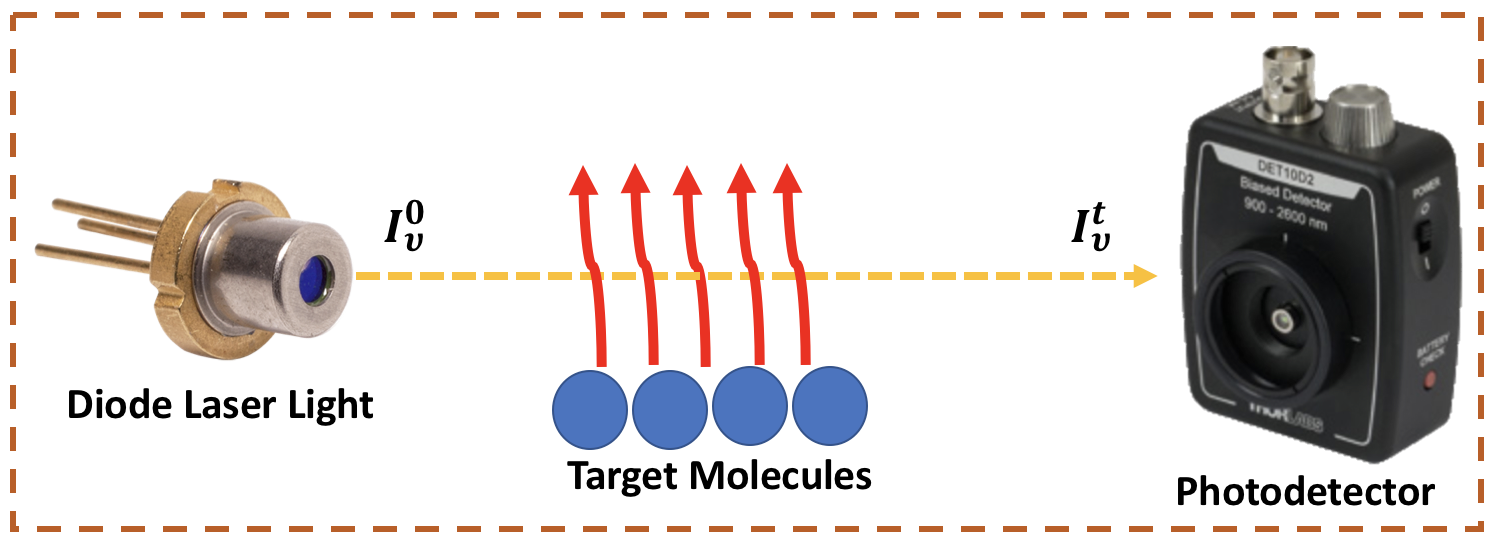
\includegraphics[width=0.7\textwidth]{fig/ch2_fig1_v2.png}
    \singlespace\caption{Schematic illustrating operating principles of line-of-sight laser-absorption spectroscopy.}
    \label{fig:ch2_1}
\end{figure}

\noindent Here, $I_\nu^0$ and $I_\nu^t$ are the incident and transmitted laser-light intensity, $k_\nu$ is the absorption coefficient [$cm^{-1}$], and L is the path length through the absorbing gas [$cm$]. The absorbance, $\alpha$, is defined as the product of $k_\nu$ and $L$. The absorbance is a function of optical frequency $\nu$, temperature $T$, gas pressure $P$, absorbing species mole fraction $\chi_i$ and path length $L$. 

%According to optically thin limit, absorbance $\alpha$ is used to describe the proportion of absorption when $\alpha$ is much less than 1.
%\begin{equation}\label{}
%1-\frac{I_\nu^L}{I_\nu^0}=1-exp(-\alpha)\approx1-(1-\alpha)=\alpha
%\end{equation}

\section{Fundamentals of Absorption Spectroscopy}
\subsection{Absorption Coefficient}
The absorption coefficient is given by:
\begin{equation}\label{}
k_v\,[cm^{-1}]=\sum_jS_{i}P\chi_i\phi_j(\nu) 
\end{equation}

\noindent Here, $S_j$ is the linestrength, $\phi_j(\nu)$ is the lineshape function, and the sum over $j$ refers to a sum over all absorption transitions that are significant at frequency $\nu$. The linestrength quantifies the probability of absorption occuring, and the lineshape function is a probability distribution function that describes how the probability of absorption occuring varies with frequency.


%Number density of molecules in state 1 and 2 reach equilibrium when the molecules leaving and entering either state is equal. Proportion of number of molecules in two energy levels can be expressed by Einstein Coefficients: $A_{21}$, $B_{12}$ and $B_{21}$, which describe spontaneous emission, induced absorption and induce emission respectively. This ratio can also be represented by Boltzmann statistical mechanics at equilibrium conditions. Absorption coefficient has the relation given by Eqn.(2.3).

%\begin{equation}\label{}
%k_v[cm^{-1}]=\frac{h\nu}{c}\frac{1}{\delta_{\nu}}[n_2B_{21}-n_1B_{12}]=\frac{h\nu}{c}\frac{1}{\delta_{\nu}}n_1B_{12}(1-exp(-h\nu/kT))
%\end{equation}

%\noindent $h$ is Planck's constant. k is Boltzmann constant. $c$ is light speed. $n_1$ and $n_2$ represent number density of molecules in state 1 and 2. $B_{12}$ stands for probabilities that molecules in state 1 will absorb a quantum and move to state 2 and vice versa for $B_{21}$. In reality, the transition spectra has a certain shape, which is described by normalized lineshape function %$\phi(\nu)$. Therefore,
%\begin{equation}\label{}
%k_v[cm^{-1}]=\frac{h\nu}{c}n_1B_{12}(1-exp(-h\nu/kT))\phi(\nu)
%\end{equation}
%\begin{equation}\label{}
%S_{12}[cm^{-2}]=\frac{h\nu}{c}n_1B_{12}(1-exp(-h\nu/kT))
%\end{equation}
%\begin{equation}\label{}
%k_v[cm^{-1}]=S_{12}[cm^{-2}]\phi(\nu) \quad [cm]
%\end{equation}

%\noindent $S_{12}$ is defined to quantify the absorption transition at frequency $\nu$ and called "line strength". 

\subsection{Linestrength}
In LAS, it is common to define the linestrength in pressure-normalized form [$cm^{-2}atm^{-1}$], however, a per-unit-number-density unit is used in the HITRAN and HITEMP database [$cm^{-1}/(molecule \, cm^{-2})$] \cite{2013JQSRT.130....4R}. Linestrength scales with the number density of molecules in the absorbing quantum state ($n_1$), and the Einstein-B coefficient for stimulated absorption. The number density in the absorbing state can be determined as a function of temperature from Boltzmann statistics and the Einstein-B coefficient can be measured experimentally (using LAS) or taken from spectroscopic databases (e.g. HITRAN). Typically, the linestrength is known at a reference temperature ($T_0$) and then the linestrength at temperature $T$ can be determined from the scaling relation by Eq.\ (\ref{eq:ch2_3}). 

\begin{equation*}
S(T)\,[cm^{-2}atm^{-1}]=S(T_0)\frac{Q(T_0)}{Q(T)}(\frac{T_0}{T})exp[-\frac{hcE^"}{k}(\frac{1}{T}-\frac{1}{T_0})] 
\end{equation*}
\begin{equation}\label{eq:ch2_3}
\quad[1-exp(\frac{-hcv_{0}}{kT})][1-exp(\frac{-hcv_{0}}{kT_0})]^{-1}  
\end{equation}

\vspace{4mm}

%\begin{equation*}
%S^n(T)=S^n(T_0)\frac{Q(T_0)}{Q(T)}exp[-\frac{hcE^"}{k}(\frac{1}{T}-\frac{1}{T_0})] 
%\end{equation*}
%\begin{equation}\label{}
%\quad[1-exp(\frac{-hcv_{0}}{kT})][1-exp(\frac{-hcv_{0}}{kT_0})]^{-1} \quad [cm^{-1}/(molec \cdot cm^{-2})]
%\end{equation}
\noindent Here, $S(T_0)$ represents the linestrength at temperature $T_0 = 296 \,K$, $Q(T)$ is the molecular partition function at temperature $T$, $E^"$ is the lower-state energy, $\nu_0$ is the frequency at the transition line center. Throughout this thesis, the linestrength is calculated using Eq.\ (\ref{eq:ch2_3}) and the absorbance spectrum of $H_2O$ transitions is calculated using Eq.\ (\ref{eq:ch2_4}). An example of simulated absorbance spectra of water transitions near 1.4 $\mu m$ is shown in Fig.\ \ref{fig:ch2_2}.

%in the demonstration and in the processing of LAS experiment data. By substituting the form of $k_\nu$ into Eqn. 2.6, absorbance at frequency of $\nu$ can be expressed by a relation in Eq.(2.4).
\begin{equation}\label{eq:ch2_4}
\alpha_\nu=\sum_jS_jP\chi_i\phi_j(\nu)L
\end{equation}

\begin{figure}[ht]
    \centering
        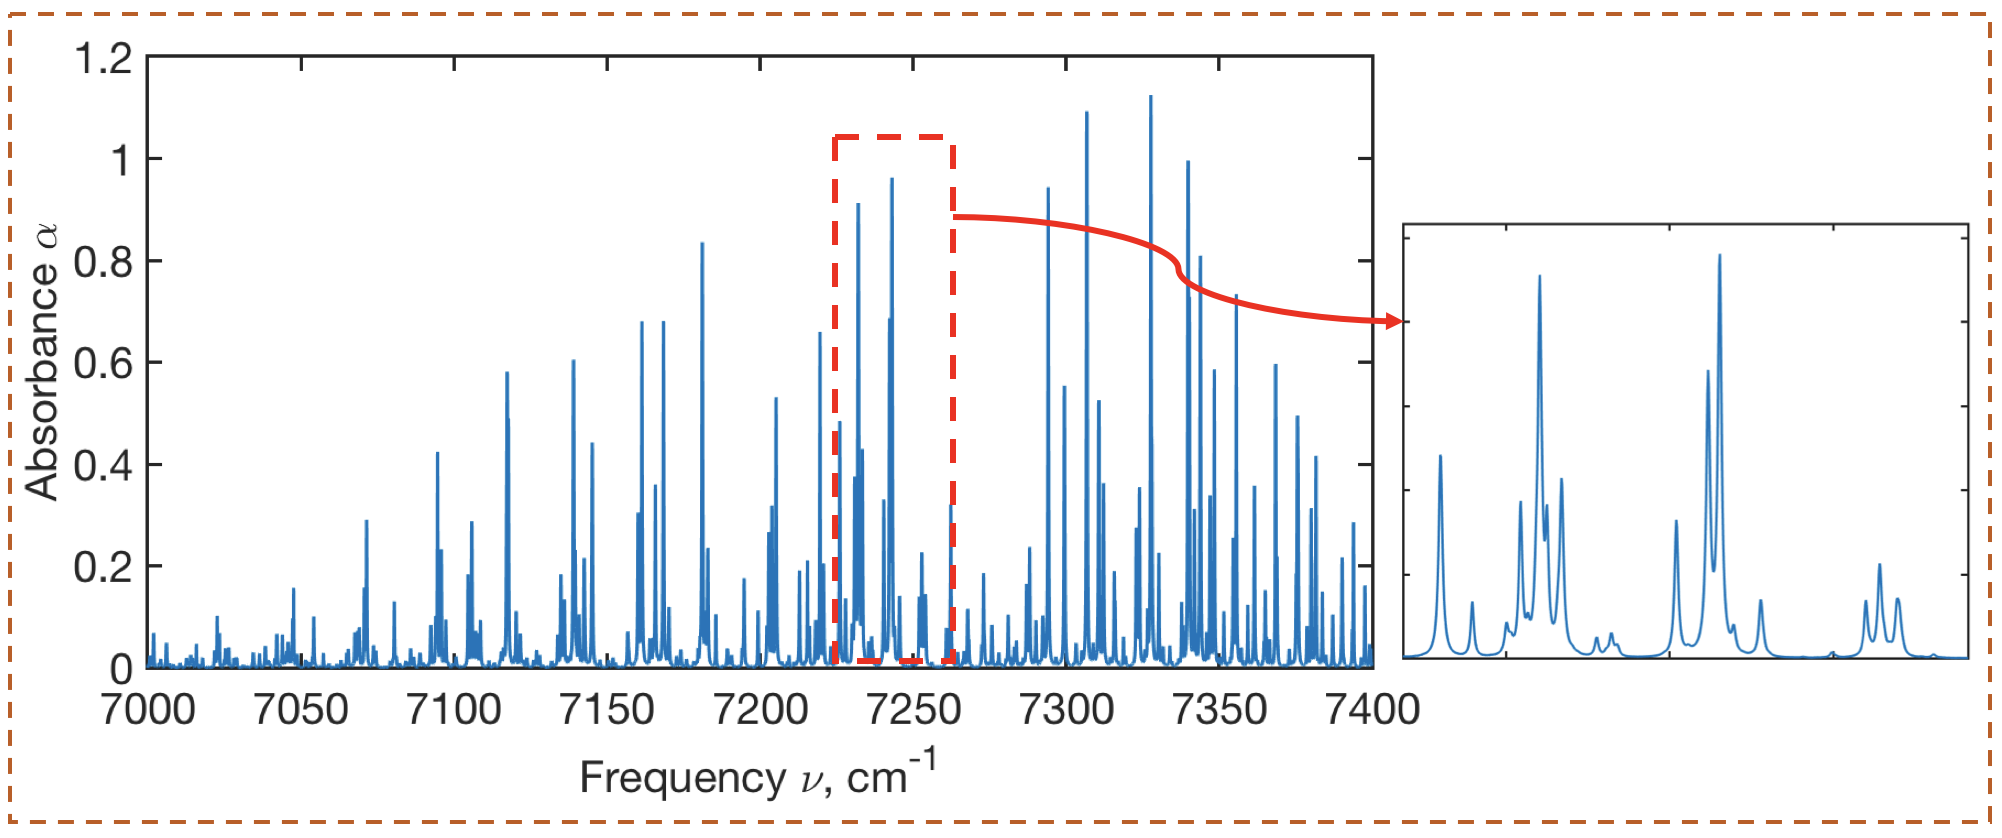
\includegraphics[width=0.85\textwidth]{fig/ch2_fig3.png}
        \caption{Simulated absorbance spectra of $H_2O$ transitions near 1.4 $\mu m$ and a zoom view over a range of 7230 $cm^{-1}$ to 7250 $cm^{-1}$. Calculations were performed for a gas temperature of 300 $K$, pressure of 1 $atm$, $H_2O$ mole fraction of 10$\%$ and path length of 10 $cm$.}
    \label{fig:ch2_2}
\end{figure}

\vspace{50mm}


\subsection{Lineshape Function}
While the linestrength describes the ``strength'' or probability of the absorption according due to a given transition, the lineshape function describes how the probability of absorption for a given transition varies as a function of frequency $\nu$. The lineshape function requires knowledge of several line-broadening mechanisms, most importantly, Doppler broadening and collisional broadening.

%absorption coefficient $k_\nu$ is the product of line strength and lineshape function, where line strength describes the absorption quantitatively and line shape indicates the absorption variation as a function of frequency $\nu$. Line shape function is characterized with line broadening mechanisms (mainly Doppler Broadening and Collisional Broadening) and line shift mechanisms (mainly pressure shift). This function has unit-normalized integration across the frequency and is maximized at its line center $\nu_0$.

Doppler Broadening results from a combination of the random thermal motion of the molecules and the Doppler effect. Molecules moving towards the photons see a higher frequency and molecules moving away from the photons see a lower frequency. The random thermal motion of molecules can be modeled using the Maxwellian velocity distribution function and this leads to a Gaussian lineshape. The Doppler full-width at half-maximum (FWHM) is given by Eq.\ (\ref{eq:ch2_5}).

%results from Doppler effects, where the radiation frequency $v_0$ shifts when molecules move in the same direction as the light with different velocities. Because molecules travel in chaos with all directions and different speeds in the space, frequency of molecules detected is closer or far from $v_0$. Statistical molecule velocity is presented in the Maxwellian velocity distribution function. Hence spectra plot as a function of frequency is broadened and the shape of spectra is known as Doppler (a.k.a Gaussian or inhomogeneous) profile. Full width at half maximum (FWHM) is an important parameter in the characterization of spectral lines. Expression of FWHM for Doppler Broadening (Doppler width) is given in Eqn. 2.10.
\begin{equation}\label{eq:ch2_5}
\Delta\nu_D \,[cm^{-1}]=v_0(\frac{8kTln2}{mc^2})^{1/2}=\nu_{0}*7.1623*10^{-7}*(\frac{T}{MW})^{1/2}
\end{equation}

\vspace{3mm}

\noindent Here, $k$ is the Boltzmann constant, $m$ is the particle mass, $c$ is the speed of light, $T$ is the temperature in $K$, and $MW$ is the molecular weight of the  target molecules in $g$/$mol$. The above equation indicates that the Doppler width is a function of molecular weight, gas temperature and the frequency of the transition. The lineshape profile due to Doppler broadening alone has a Gaussian lineshape function given by Eq.\ (\ref{eq:ch2_6}):

\begin{equation}\label{eq:ch2_6}
\phi_D(\nu) \,[cm]=\frac{2}{\Delta\nu_D}(\frac{ln2}{\pi})^{1/2}exp\{-4ln2(\frac{\nu-\nu_0}{\Delta\nu_D})^2\}
\end{equation}

\vspace{3mm}

Collisional Broadening, also called pressure broadening, results from a collision-induced uncertainty in the energy of the absorbing state. As molecules travel in the space, inelastic collisions can occur, which reduces the molecule's lifetime in a given quantum state. According to the Heisenberg uncertainty principle, this increased uncertainty in the lifetime of a molecule in a given state leads to a larger uncertainty in the energy of the quantum state. This also enables molecules to absorb photons over a range of energies/frequencies, and hence broadens the transition lineshape. If the collisional broadening is independent of the molecule's speed, the collisional broadening is homogeneous, and the lineshape can be modeled by a Lorentzian function given by Eq.\ (\ref{eq:ch2_7}). 
\begin{equation}\label{eq:ch2_7}
\phi_L(\nu) \,[cm]=\frac{1}{2\pi}\frac{\Delta\nu_C}{(\nu-\nu_0)^2+(\Delta\nu_C/2)^2}
\end{equation}
%As line width of spectra is determined by molecule lifetime, line shape is thus broadened compared with natural line width. This type of spectra shape is called Lorentzian profile or homogeneous profile. Expression of FWHM for Collisional Broadening is given in Eqn. 2.12.

\vspace{3mm}

\noindent The collisional FWHM ($\Delta\nu_C$) is given by Eq.\ (\ref{eq:ch2_8}).
\begin{equation}\label{eq:ch2_8}
\Delta\nu_C \,[cm^{-1}]=\sum_A Px_A2\gamma_{B-A} 
\end{equation}

\noindent Here, $B$ is the absorbing molecule, $A$ represents a set of collisional partners of $B$ in the test gas, $P$ is pressure in the unit of $atm$, $x_A$ is the mole fraction of species $A$, and $2\gamma_{B-A}$ is the collisional-broadening coefficient. The temperature scaling of $\gamma_{B-A}$ can often be modeled using:
\begin{equation}\label{}
\gamma_{B-A}(T)=\gamma_{B-A}(T_0)*(T/T_0)^{n}
\end{equation}

%Broadening coefficient is temperature-dependent because temperature is related to thermal motions of molecules.
\noindent where, $n$ is the temperature scaling exponent which can be found in spectroscopic databases or measured experimentally. Hence the collisional width is a function of pressure, temperature and properties of collisional partners.

\vspace{2mm}

\begin{table}[h]
\begin{center}
\begin{tabular}{ c c c }
\hline
Species & Wavelength $[cm^{-1}]$ & air-broadened coefficient $[cm^{-1}/atm]$\\ \hline
$H_2O$ & 7183.9 & 0.039\\ 
$H_2O$ & 7446.1 & 0.067\\ 
$CO$ & 2059.9 & 0.055\\ \hline
\end{tabular}
\caption{Examples of collisional-broadening coefficient 2$\gamma$ [$cm^{-1}/atm$] in air at 296 $K$. Data taken from the HITRAN 2012 database \cite{2013JQSRT.130....4R}.}
\label{table:ch2_1}
\end{center}
\end{table}

\vspace{-5mm}

Table 2.1 shows some broadening coefficients of $H_2O$ and $CO$ transitions at 296 $K$ and 1 $atm$. These data are taken from the HITRAN 2012 database \cite{2013JQSRT.130....4R}.

%In this thesis, $H_2O$ serves as the target molecule. Accordingly collisional width has a form: 
%\begin{equation}\label{}
%\Delta\nu_C=P*(x*\gamma_{self,T}+(1-x)*\gamma_{air,T})
%\end{equation}
%Where $\gamma_{self}$ and $\gamma_{air}$ are self- and air-broadening coefficients available from HITRAN.

%As mentioned above, collisions between molecules result in intermolecular energy transfer and thus change of their fundamental frequencies for transitions. Because collision width is a function of pressure (Eqn. 2.12), this spectra line shift is known as pressure shift given by Eqn. 2.15. 
%\begin{equation}\label{}
%\Delta\nu_S=\sum_A Px_A\delta_A \quad [cm^{-1}]
%\end{equation}
%\begin{equation}\label{}
%\delta_{T}=\delta_{T_0}*(T/T_0)^{m}
%\end{equation}

%A is a set of collisional partners of target molecule. $\delta_A$ is shift coefficient. Similar as collisional width coefficient, this parameter is also temperature-dependent and the expression is given in Eqn. 2.17. $m$ is temperature coefficient. For $H_2O$ molecule in the air, shifted line center frequency can be written as:
%\begin{equation}\label{}
%\nu_{0,s}=\nu_{0}+\delta_{air}*(T/T_0)^mP(1-x)
%\end{equation}

\subsection{Voigt Profile}
At conditions relevant to most combustion gases, Doppler broadening and collisional broadening are both significant. In this case, the Voigt function is typically used to model the lineshape function. The Voigt function is given by a convolution of the Lorentzian and Doppler profiles:

\begin{equation}\label{eq:ch2_10}
\phi_V(\nu)=\int_{-\infty}^{\infty}\phi_D(u)\phi_L(\nu-u)du=\phi_D(\nu_{0})V(a,w)
\end{equation}

\noindent where,

\begin{equation}\label{}
a=\frac{\sqrt[]{ln\,2}\Delta\nu_C}{\Delta\nu_D}
\end{equation}

\begin{equation}\label{}
w=\frac{2\,\sqrt[]{ln\,2}\nu-\nu_{0}}{\Delta\nu_D}
\end{equation}

\begin{equation}\label{eq:ch2_13}
\phi_D(\nu_{0})=\frac{2}{\Delta\nu_D}\,\sqrt[]{\frac{ln\,2}{\pi}}
\end{equation}

\vspace{3mm}

\noindent $V(a,w)$ is known as the Voigt function, where parameter $a$ quantifies the relative effect on the line profile from collisional and Doppler broadening, and parameter $w$ is a measure of the distance from linecenter. As shown from Eq.\ (\ref{eq:ch2_10}) to Eq.\ (\ref{eq:ch2_13}), the Voigt profile is a function of linecenter frequency, collisional width and Doppler width. Hence the line shape function can be expressed as:

\begin{center}
$\phi(\nu_{0},\Delta\nu_D,\Delta\nu_C)$
\end{center}

Therefore, the expression of absorbance has the following form:
\begin{equation}\label{}
\alpha(\nu)=\sum_{transitions, j}S_j(T)P\chi_{i,species}\phi_{\nu,j}(\nu_{0,j},\Delta\nu_{D,j},\Delta\nu_{C,j})
\end{equation}

\begin{figure}[b]
    \centering
        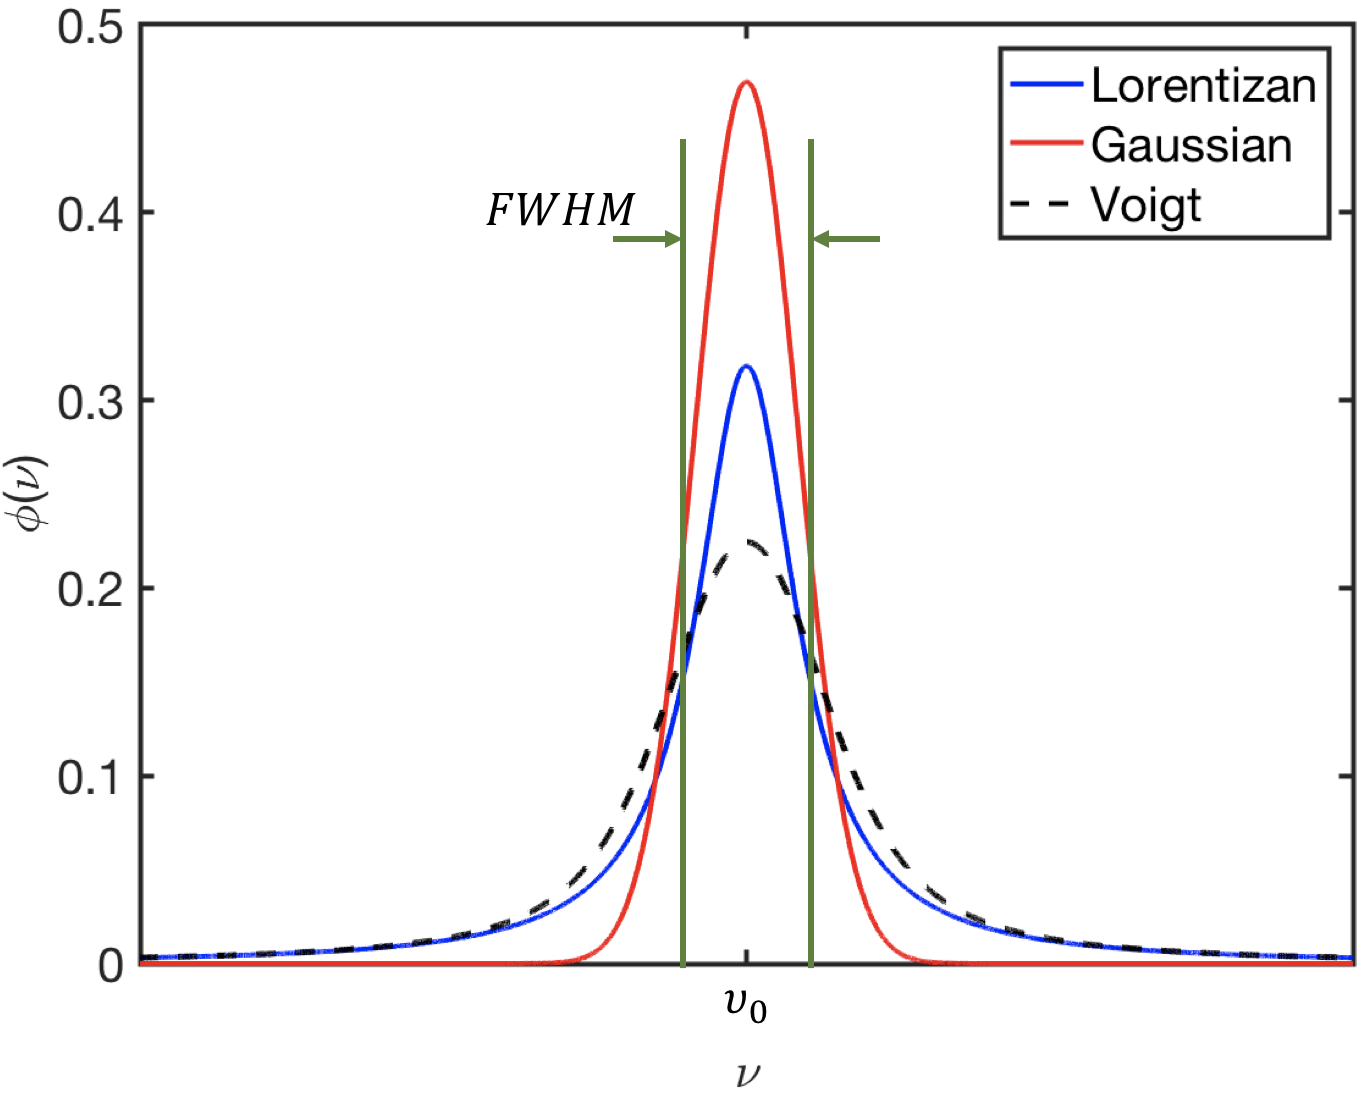
\includegraphics[width=0.6\textwidth]{fig/ch2_fig4.png}
        \caption{Comparison of simulated Lorentzian, Gaussian and Voigt lineshapes with $\Delta\nu_C=\Delta\nu_D$.}
    \label{fig:ch2_3}
\end{figure}

Fig.\ \ref{fig:ch2_3} compares Lorentzian (collisional), Gaussian (Doppler) and Voigt lineshapes. In this figure, Lorentzian and Gaussian profiles are simulated with the same FWHM, but the Gaussian profile has a larger peak amplitude and decreases more rapidly away from the linecenter while the Lorentzian profile has larger wings. This indicates that these broadening mechanisms affect the line shape differently and that the Voigt profile is required to account for both of these effects.

%and both are significant for the accuracy of the lineshape simulation. Voigt profile is the combination of the two. It has been widely used with great computational efficiency in multiple applications such as the combustion measurements presented in Chapter 4.

\section{Direct Absorption Techniques}
%Based on Beer's Law (Eqn. 2.1.), this technique is simple but functional. In fixed-wavelength DA, laser beam is transmitted from sources without being scanned (or tuned).
Fixed-wavelength direct absorption (DA) is the simplest laser-absorption diagnostic technique. In this method, the laser light is resonant (at a fixed frequency) with an absorption transition and directed through a test gas onto a detector. Any change in the transmitted light intensity ($I_\nu^t$) is assumed to result from absorption by the target species. As a result, the absorption signal can be detected with a very high bandwidth (MHz), set by the detector bandwidth or sampling rate. For this reason, this technique is frequently used to resolve reaction kinetics in shock tubes \cite{HANSON2014103}. While simple, this technique can suffer from major drawbacks that cannot be easily identified in an experiment. For example, many other factors can decrease or increase the amount of light collected by the photodetector (e.g., beamsteering, background emission), which can lead to large errors in the perceived measurement of absorbance. In addition, the laser frequency may become unstable and lead to errors in interpreting the measured absorbance. 

Scanned-wavelength DA is a more robust technique. By tuning the injection current of a diode laser, the laser frequency can be scanned across an absorbance transition to provide a measurement of the absorption spectrum. Laser light travels through the test gas onto a photo-detector. An etalon is used to determine how the wavelength varies in response to current modulation. By taking a ratio of incident and transmitted light intensity, absorbance as a function of wavelength can be obtained. If individual absorption transitions are resolved, the integrated absorbance, $A$, can be obtained which is directly related to linestrength, pressure and path length (Eq.\ (\ref{eq:ch2_15})) and independent of the transition lineshape. That also indicates that if two laser are applied at the same time, the ratio of integrated absorbance for two lines can be determined which is only a function of temperature (Eq.\ (\ref{eq:ch2_16})). Hence temperature can be determined from the two-color ratio of integrated absorbance, R, given by Eq.\ (\ref{eq:ch2_17}).
%Absorption signal is able to be detected with high bandwidth at the rate of sampling rate, so fix-wavelength DA can achieve fast measurements and be applied in blast measurements, for example. Drawback of this technique is that laser frequency may become unstable for long-time measurements. Instead, scan-wavelength DA behaves more robust. 
\vspace{-2mm}
\begin{equation}\label{eq:ch2_15}
A_{int}=S(T)\times P \times \chi \times L \times \int_{-\infty}^{\infty}\phi(\nu) \cdot dv=S(T) \times \chi \times P \times L
\end{equation}
\vspace{-2mm}

\begin{equation}\label{eq:ch2_16}
R(T)=\frac{A_1}{A_2}=\frac{S_1(T)}{S_2(T)}
\end{equation}

\vspace{-2mm}
\begin{equation}\label{eq:ch2_17}
T=\frac{\frac{hc}{k}(E_2^"-E_1^")}{ln\,(A_1/A_2)+ln\,(\frac{S_2(T_0)}{S_1(T_0)})+\frac{hc}{kT_0}(E_2^"-E_1^")}
\end{equation}

\vspace{5mm}

Once the gas temperature is obtained, the absorbing species mole fraction can be calculated from the measured integrated absorbance of either transition (Eq.\ (\ref{eq:ch2_18})).
\begin{equation}\label{eq:ch2_18}
\chi=\frac{A_{int}}{S(T)PL}
\end{equation}

Fig.\ \ref{fig:ch2_4} illustrates the key steps associated with a scanned-DA experiment. The measured light intensity is curve-fitted with $3^{rd}$-order polynomial to non-absorbing regions in order to determine the incident light intensity \textit{in situ}. Beer's Law is then used to calculate the measured absorbance spectrum and Voigt profiles are fit to the measured spectrum to determine the integrated absorbance of each transition (see Fig.\ \ref{fig:ch2_4}(b)). Temperature can then be inferred using Eq.\ (\ref{eq:ch2_16}) and Eq.\ (\ref{eq:ch2_17}). The above process can be repeated to acquire a time history of temperature in an experiment. 

\begin{figure}[h]
    \centering
        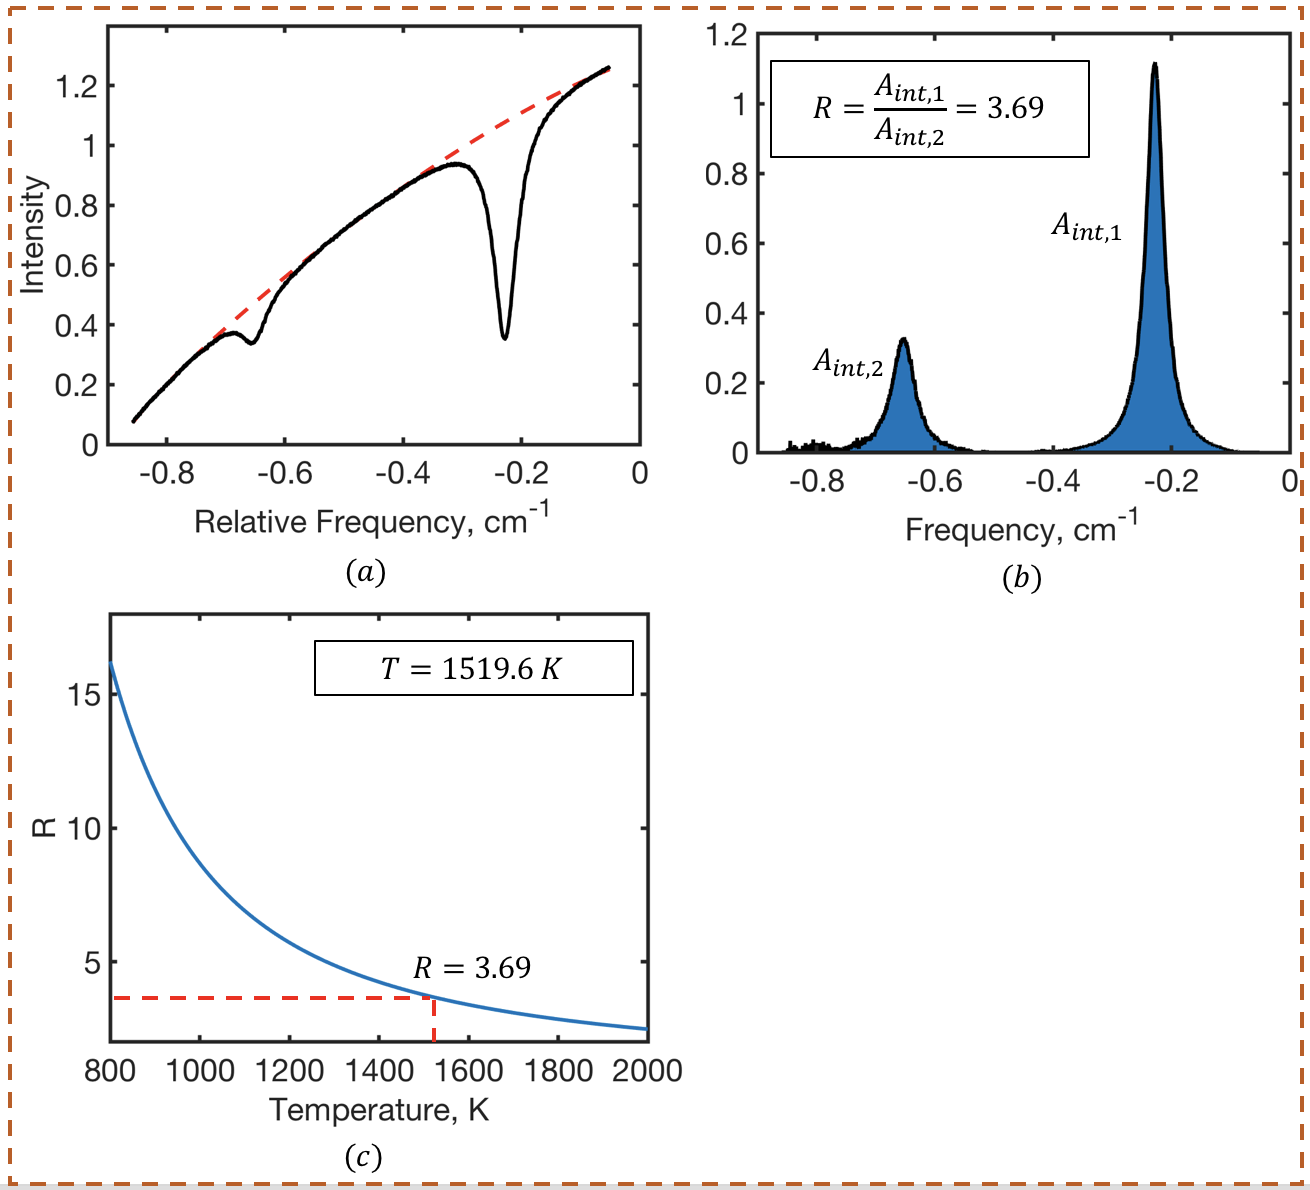
\includegraphics[width=0.7\textwidth]{fig/ch2_fig2_v3.png}
        \caption{Example of Scanned-wavelength DA measurement near 4.85 $\mu m$ for CO and temperature measurements in a $C_2H_4$-$air$ diffusion flame. (a) transmitted signal and baseline-fitted incident intensity; (b) absorbance spectra for both transitions and the two-color ratio of integrated absorbance, $R$; (c) $R$ as a function of temperature.}
    \label{fig:ch2_4}
\end{figure}


Scanned-wavelength DA exhibits several significant advantages compared to fixed-wavelength DA. First, the integral of line profile function is unit-normalized, determination of temperature and absorbing species mole fraction does not require knowledge of the lineshape broadening parameters. Second, by performing wavelength and intensity scanning, the incident light intensity can be inferred $in\,situ$ from baseline fitting, thereby accounting for non-absorbing transmission losses. However, scanned-wavelength DA can suffer from low signal-to-noise ratio (SNR) in harsh environments that produce low optical throughputs and strong beamsteering-induced noise. When the transmitted light-intensity is small, electronic noise can cause the SNR for scanned-wavelength DA to be low and fluctuate significantly, and make it difficult to accurately measure small absorbance signals. To overcome these problems, wavelength modulation spectroscopy (WMS) was used, and will be discussed in the next chapter.

%has a drawback about measurement accuracy. Accurate LAS measurements rely on the signal quality from detectors and other electrical instruments. Signal-to-Noise ratio (SNR) is an important indicator to evaluate measurement quality, which is the ratio of mean signal power over standard deviation intensity in the noise. When the signal power is not large, SNR for scan-wavelength DA can fluctuate significantly. That results from (1) baseline fitting and (2) beam steering and scattering. As shown in Fig 2.2, incident intensity is curve-fitted with high-order polynomials based on transmitted intensity. However in some applications, it is difficult to identify and curve-fit signal due to some overlaps between transitions and their neighbors. Another source to affect SNR of DA is beam steering or scattering. That leads to attenuations of detected signals and thus make measurements of transmitted intensity of baseline-fitting of incident intensity inaccurate.

